\documentclass[conference]{IEEEtran}

% Packages
\usepackage[utf8]{inputenc}
\usepackage[english]{babel}
\usepackage{amsmath}
\usepackage{amsfonts}
\usepackage{amssymb}
\usepackage{amsthm}
\usepackage{pdfpages}
\usepackage{graphicx}
\usepackage{epstopdf}
\usepackage{listings}
\usepackage{cite}
\usepackage{enumerate}
\usepackage{scientific}
\usepackage[colorlinks=false]{hyperref}
\usepackage{bookmark}

\usepackage[]{mcode}	%Matlab Code
\usepackage{tikz,pgfplots}	%Tikz

% Bookmark Setup
\bookmarksetup{numbered}

% PDF Setup
\hypersetup{pdftitle={Homework 2}, pdfsubject={Documentation of 1st Homework}, pdfauthor={Stefan Röhrl}, pdfkeywords={Neuroprothetik Exercise}, pdfcreator={LaTeX}, hidelinks}


\begin{document}
%
% cite all references
%\nocite{*}
%
% paper title
% can use linebreaks \\ within to get better formatting as desired
\title{Homework 2\\ Mathematical Basics 1}

\author{\IEEEauthorblockN{Stefan Röhrl}
\IEEEauthorblockA{Technische Universität München, Arcisstraße 21, Munich, Germany\\
Email: stefan.roehrl@tum.de}}

% use for special paper notices
%\IEEEspecialpapernotice{(Invited Paper)}

% make the title area
\maketitle

\IEEEpeerreviewmaketitle

\section{Plot slope fields and isocline}
In Abb. \ref{fig:fkt1} ist das Richtungsfeld und die Isoklinen der Differentialgleichung \ref{eq:dgl1} aufgezeichnet. Egal ein welchem Punkt man startet man landet auf der Isoklinen mit $\frac{dV}{dt}=-1$.
\begin{equation}
	\frac{dV}{dt} = 1 - V - t
	\label{eq:dgl1}
\end{equation}
\begin{figure}
	\centering
	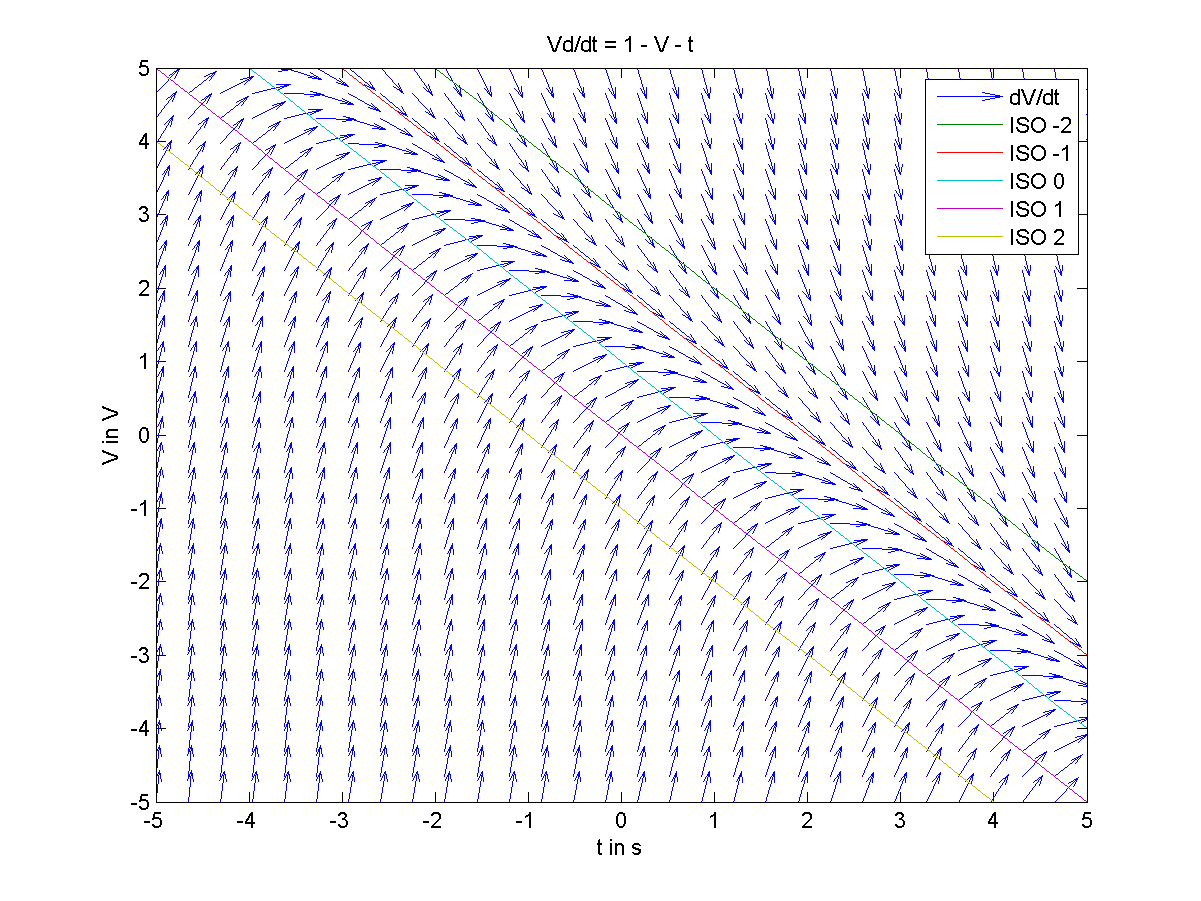
\includegraphics[width=0.5\textwidth]{img/fkt1.png}
	\caption{Richtungsfeld der Differentialgleichung (1)}
	\label{fig:fkt1}
\end{figure}

In Abb. \ref{fig:fkt2} ist das Richtungsfeld und die Isoklinen der Differentialgleichung \ref{eq:dgl2} aufgezeichnet. 
\begin{equation}
	\frac{dV}{dt} = sin(t) - \frac{V}{1.5}
	\label{eq:dgl2}
\end{equation}
\begin{figure}
	\centering
	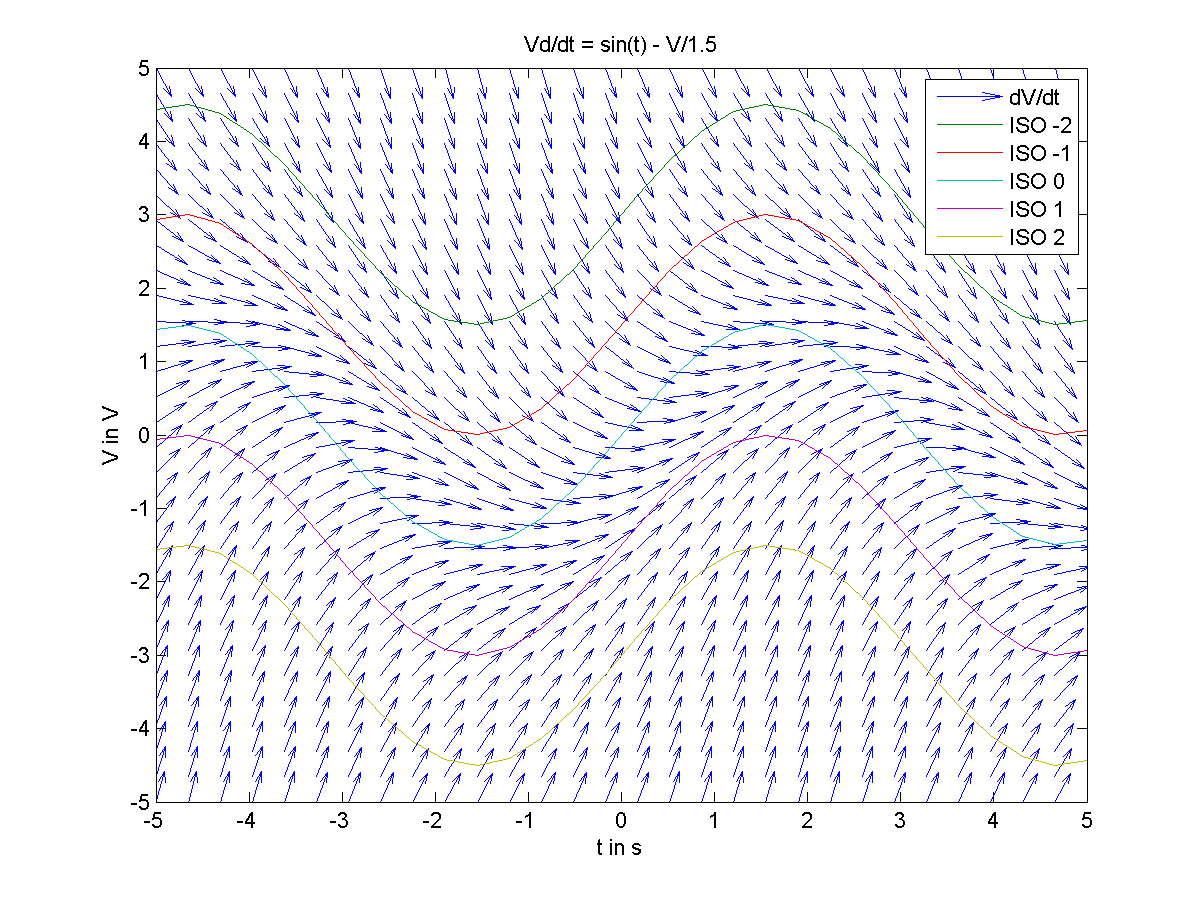
\includegraphics[width=0.5\textwidth]{img/fkt2.png}
	\caption{Richtungsfeld der Differentialgleichung (2)}
	\label{fig:fkt2}
\end{figure}

\section{Differential equations of a simple cell model}
Die Differentialgleichung für das "leaky integrate and fire neuron" erschließt sich folgendermaßen:
\begin{align}
I_{ex}  & = I_{C_m} + I_{R_l}\\
I_{C_m} & = C_m \cdot \frac{dV}{dt}\\
I_{R_l} & = \frac{V}{R_l}\\
I_{ex}  & = C_m \cdot \frac{dV}{dt} + \frac{V}{R_l}\\
\frac{dV}{dt} & = \frac{1}{C_m}(I_{ex} - \frac{V}{R_l})
\label{dgl}
\end{align}
Mit der Definition von $I_{ex} = I_{max} sin(t)$ und einem zusätzlichen konstanten Strom D ergibt sich für die Differentialgleichung diese Form:
\begin{equation}
	\frac{dV}{dt} = \frac{1}{C_m}(I_{max} sin(t) + D - \frac{V}{R_l})
\end{equation}

\newpage
In den folgenden Betrachtungen gilt: $R_l=1\Omega$, $C_m=1F$\\
In Abb. \ref{fig:slope1} ist zu erkennen, dass wenn kein externer Strom anliegt, die Zelle immer auf ein Potential von 0V zurück kehrt. Dies geschieht durch den Leck-Strom durch den Widerstand $R_l$.
\begin{figure}[h!]
	\centering
	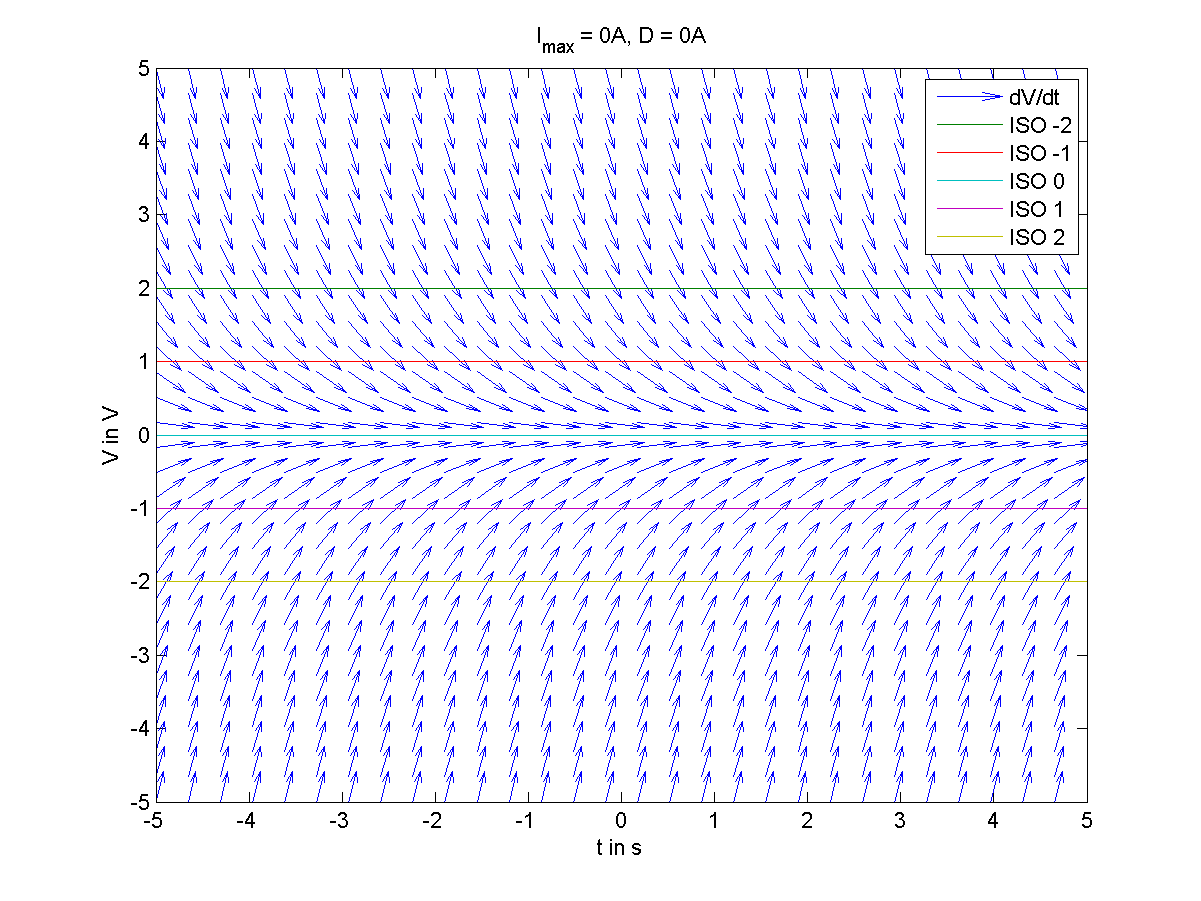
\includegraphics[width=0.5\textwidth]{img/slopefield1.png}
	\caption{Richtungsfeld mit $I_{max}=0A$, $D=0A$}
	\label{fig:slope1}
\end{figure}

In Abb. \ref{fig:slope2} ist zu sehen, wie sich die Zelle verhält wenn ein sinusförmiger Strom eingeprägt wird. 
\begin{figure}[h!]
	\centering
	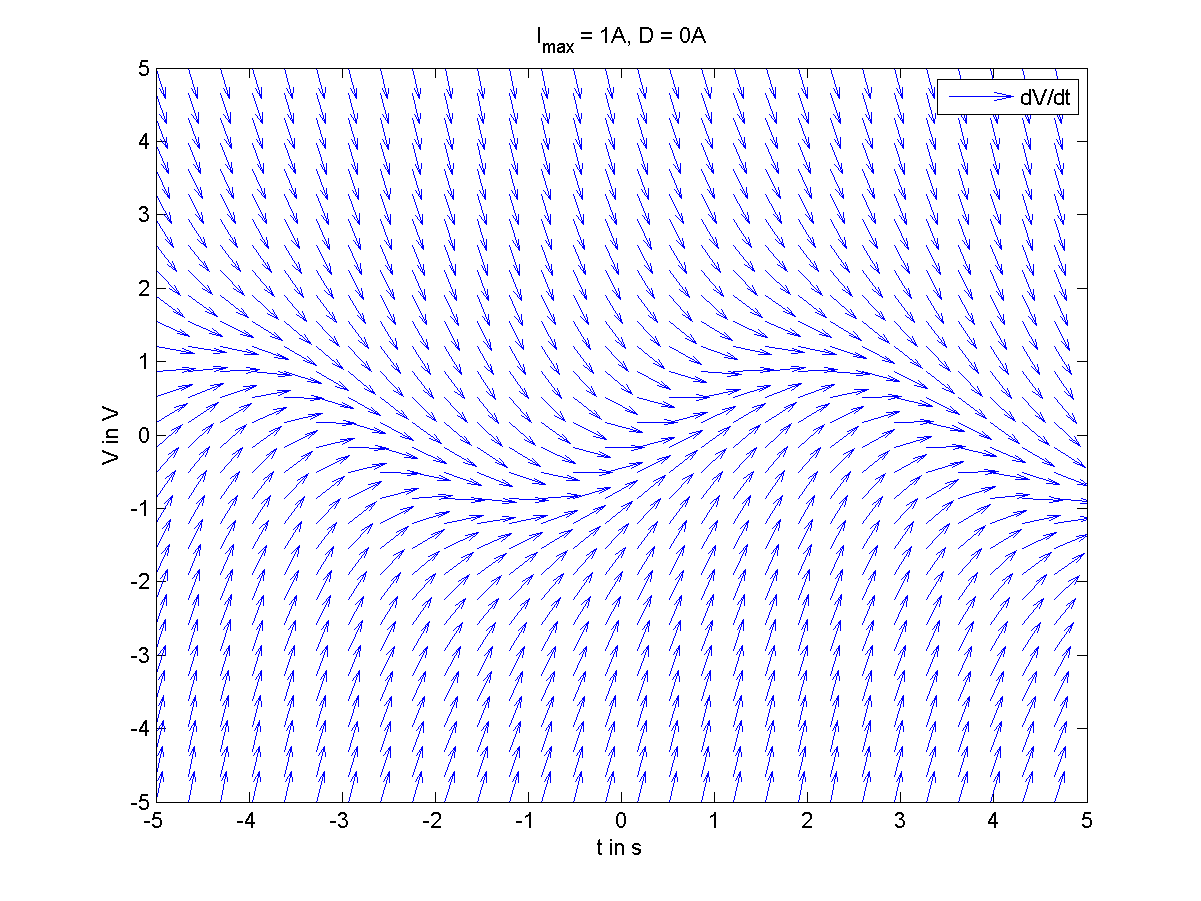
\includegraphics[width=0.5\textwidth]{img/slopefield2.png}
	\caption{Richtungsfeld mit $I_{max}=1A$, $D=0A$}
	\label{fig:slope2}
\end{figure}

Der externe konstante Strom in Abb. \ref{fig:slope3} sorgt dafür, dass sich die Zelle unter eine Vorspannung befindet. Der Kondensator wird soweit aufgeladen bis der komplette Strom über $R_l$ abfließt. Somit wird das Potential konstant bei 2V gehalten. Wird die Zelle auf ein anderes Potential angeregt, kehrt sie wieder zum 2V Potential zurück.\\
\begin{figure}[h!]
	\centering
	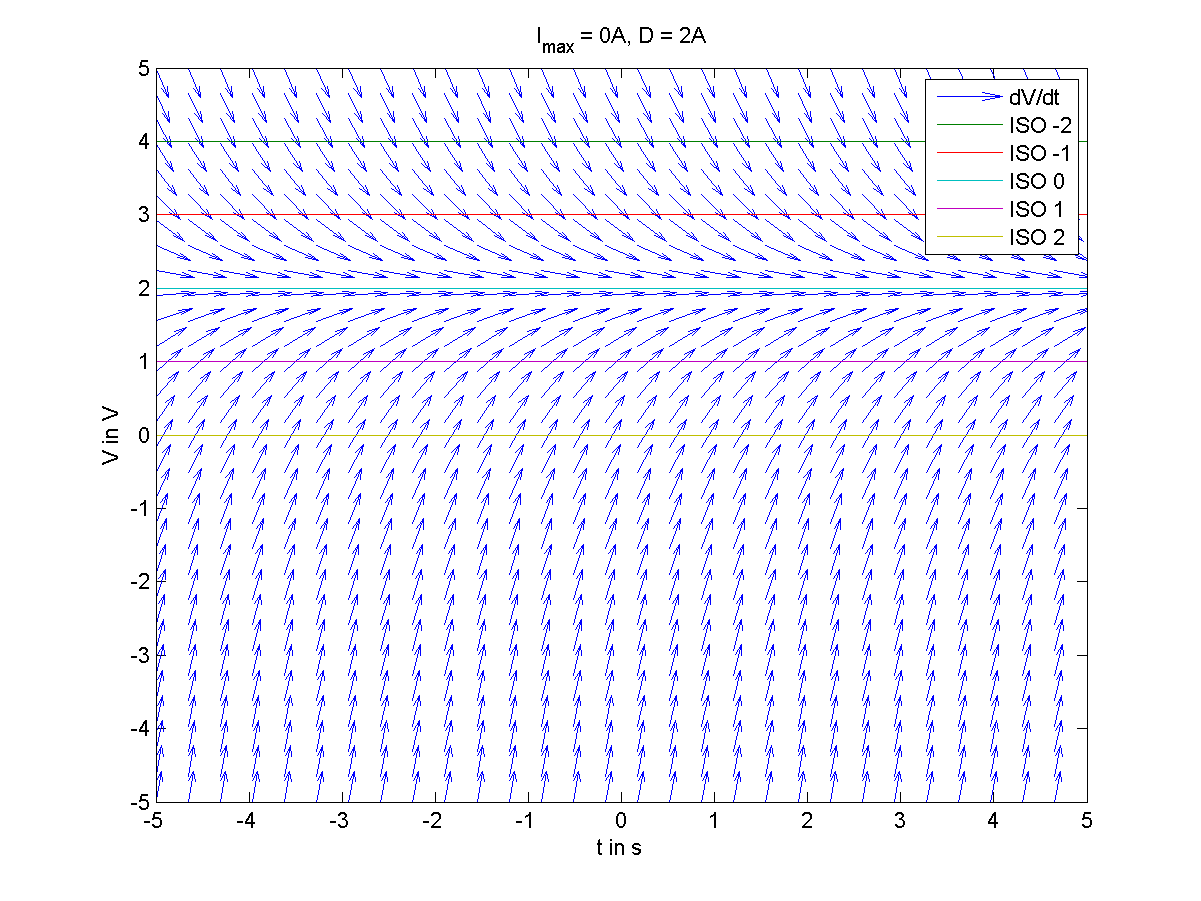
\includegraphics[width=0.5\textwidth]{img/slopefield3.png}
	\caption{Richtungsfeld mit $I_{max}=0A$, $D=2A$}
	\label{fig:slope3}
\end{figure}

Wird nun zusätzlich ein sinusförmiger Strom eingeprägt schwingt die Zelle um das 2V Potential (vgl. Abb. \ref{fig:slope4}).
\begin{figure}[h!]
	\centering
	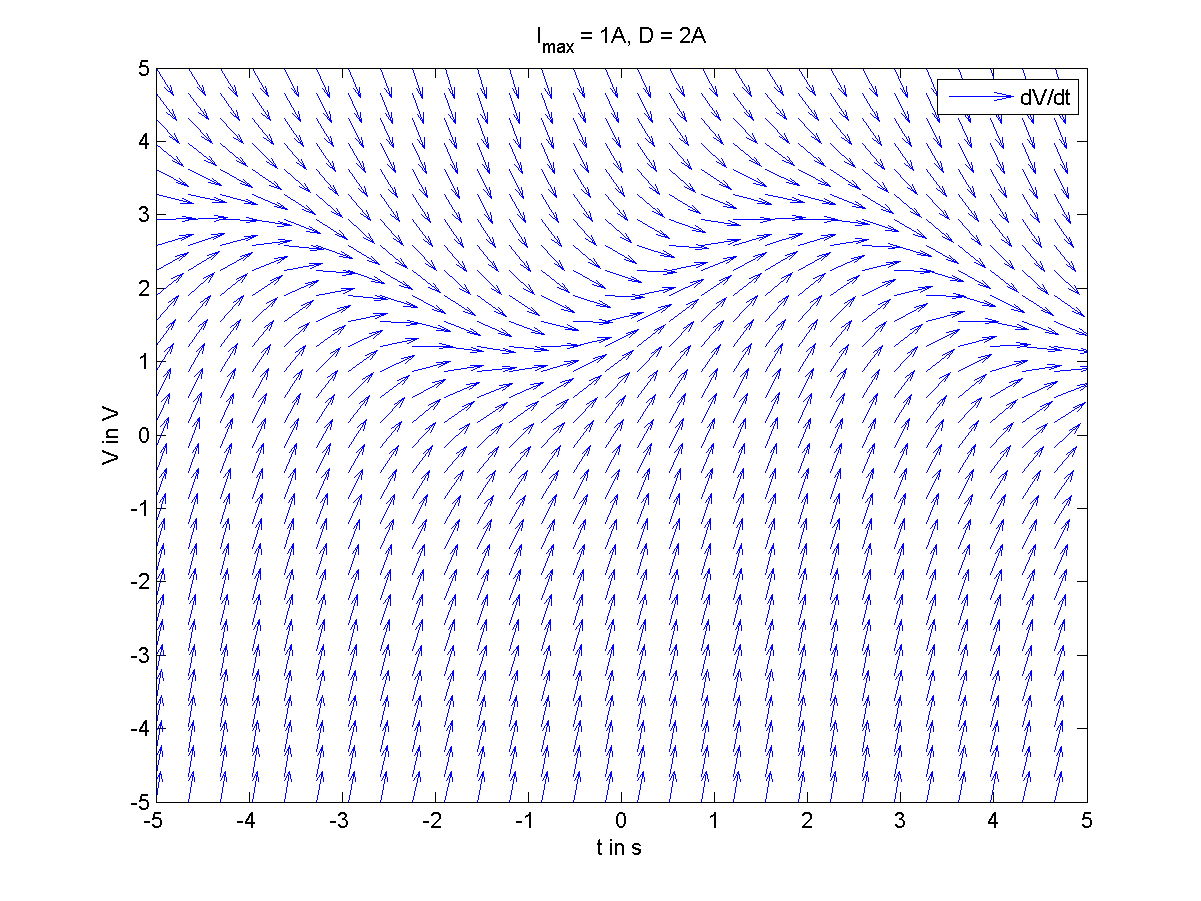
\includegraphics[width=0.5\textwidth]{img/slopefield4.png}
	\caption{Richtungsfeld mit $I_{max}=1A$, $D=2A$}
	\label{fig:slope4}
\end{figure}

\end{document}


